\documentclass[12pt]{article}
\textwidth=16.00cm
\textheight=22.00cm
\topmargin=0.00cm
\oddsidemargin=0.00cm
\evensidemargin=0.00cm
\headheight=0cm 
\headsep=0.5cm
%%%%%%%%%%%%%%%%%%%%%%%%%%%%%%%%%%%%%%%%%%%%%%%%%%%%%%%%%%%%%%%
\usepackage{amsmath}
\usepackage[utf8]{inputenc}
\usepackage[american]{babel}
\usepackage{amssymb}
\usepackage{graphicx}
\usepackage{caption}
\usepackage{tikz}
\usepackage{float}
\usepackage{amsthm}
\usetikzlibrary{patterns}
%%%%%%%%%%%%%%%%%%%%%%%%%%%%%%%%%%%%%%%%%%%%%%%%%%%%%%%%%%%%%%%
\newtheorem{theorem}{Theorem}[section]
\newtheorem{lemma}[theorem]{Lemma}
\newtheorem{conjecture}[theorem]{Conjecture}
\newtheorem{proposition}[theorem]{Proposition}
\newtheorem{corollary}[theorem]{Corollary}
\newtheorem{remark}[theorem]{Remark}
\newtheorem{definition}[theorem]{Definition}
\theoremstyle{definition}
\newtheorem{example}[theorem]{Example}
%%%%%%%%%%%%%%%%%%%%%%%%%%%%%%%%%%%%%%%%%%%%%%%%%%%%%%%%%%%%%%%
\newcommand{\claim}[2]{\textit{Claim #1. #2: }}
%%%%%%%%%%%%%%%%%%%%%%%%%%%%%%%%%%%%%%%%%%%%%%%%%%%%%%%%%%%%%%%
%\parskip 6pt
%\addtocounter{section}{-1}
%%%%%%%%%%%%%%%%%%%%%%%%%%%%%%%%%%%%%%%%%%%%%%%%%%%%%%%%%%%%%%%
\title{Goldbach Conjecture}
\author{Matthew Watson}
%%%%%%%%%%%%%%%%%%%%%%%%%%%%%%%%%%%%%%%%%%%%%%%%%%%%%%%%%%%%%%%
\newcommand{\N}{\mathbb{N}}
\newcommand{\Z}{\mathbb{Z}}
\renewcommand{\P}{\mathbb{P}}
%%%%%%%%%%%%%%%%%%%%%%%%%%%%%%%%%%%%%%%%%%%%%%%%%%%%%%%%%%%%%%%%%%%%%%%%%%%%%%%%%%%%%%%%%%%%%%%%%%%
\begin{document}
%%%%%%%%%%%%%%%%%%%%%%%%%%%%%%%%%%%%%%%%%%%%%%%%%%%%%%%%%%%%%%%%%%%%%%%%%%%%%%%%%%%%%%%%%%%%%%%%%%%
\section{Introduction}
\label{sec:intro}
%%%%%%%%%%%%%%%%%%%%%%%%%%%%%%%%%%%%%%%%%%%%%%%%%%%%%%%%%%%%%%%%%%%%%%%%%%%%%%%%%%%%%%%%%%%%%%%%%%%
\begin{proposition}[Goldbach Conjecture]
\label{prop:GC}
Every even integer greater than 2 is the sum of two primes.
\end{proposition}

The Goldbach Conjecture is equivalent to the following.

\begin{proposition}
Every integer $n \geq 2$ is the average of two primes.
\end{proposition}

A natural extension of the Goldbach conjecture is the following.

\begin{proposition}
If a prime $p$ divides an integer $n \geq 2$, then $n$ is the average of $p$ primes.
\end{proposition}

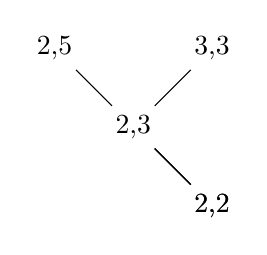
\begin{tikzpicture}
	\node (22) at (0,0)		{2,2};
	
	\node (23) at (-1,1)	{2,3};
	\node (25) at (-2,2)	{2,5};
	
	\node (33) at (0,2)		{3,3};
	\node (2,2) at (0,0)	{2,2};
	
	\path [-] (22) edge (23);
	\path [-] (23) edge (33);
	\path [-] (23) edge (25);
	\path [-] (22) edge (23);
	\path [-] (22) edge (23);
\end{tikzpicture}

Another equivalent statement due to Sebastian Mart{\'i}n Ruiz is as follows.

\begin{proposition}
\label{prop:SMR}
For all even integers $n \geq 4$, there exists an integer $k \in [n-1]$ such that
\[
\varphi(n^2 - k^2) = (n-1)^2 - k^2.
\]
\end{proposition}

\begin{proposition}
Proposition \ref{prop:SMR} is equivalent to the Goldbach Conjecture.
\end{proposition}

\begin{proof}
Suppose $e \geq 4$ is an even integer.

If the Goldbach Conjecture is true, then there exist two primes $p$ and $q$ such that $e = p + q$, and without loss of generality, we can suppose $p > q$. Let $n := (p + q)/2$ and $k := (p - q)/2$.

Now, 

\begin{align*}
  \varphi(n^2 - k^2) & = \varphi((n + k)(n - k)) \\
                     & = \varphi(pq) \\
                     & = \varphi(p)\varphi(q) \\
                     & = (p - 1)(q - 1) \\
                     & = ((n + k) - 1)((n - k) - 1) \\
                     & = ((n - 1) + k)((n - 1) - k) \\
                     & = (n - 1)^2 - k^2
\end{align*}

Conversely, if \ref{prop:SMR} holds, then there exists an integer $k \in [n-1]$ such that 
\[
\varphi(n^2 - k^2) = (n-1)^2 - k^2.
\]

Let $n := e/2$. If $n + k$ and $n - k$ are both prime, then we are done by setting $p := n + k$ and $q := n - k$. Otherwise, at least one of $n + k$ or $n - k$ is composite. Let $d := gcd(n + k, n - k)$. Then we arrive at the contradiction $\varphi(n^2 - k^2) < (n - 1)^2 - k^2$:

\begin{align*}
  \varphi(n^2 - k^2) & = \varphi((n + k)(n - k)) \\
                     & = \varphi\Big(d^2\frac{(n + k)}{d}\frac{(n - k)}{d}\Big) \\
                     & = \varphi(d^2)\varphi\Big(\frac{n + k}{d}\frac{n - k}{d}\Big) \\
                     & = d\varphi(d)\varphi\Big(\frac{n + k}{d}\Big)\varphi\Big(\frac{n - k}{d}\Big) \\
                     & = d\varphi\Big(\frac{n + k}{d}\Big)\varphi(d)\varphi\Big(\frac{n - k}{d}\Big) \\
                     & \leq \varphi\Big(d\frac{n + k}{d}\Big)\varphi\Big(d\frac{n - k}{d}\Big) \text{\ \ \ \ \ \ \ \ \ \ (equality if $d=1$)}\\
                     & = \varphi(n + k)\varphi(n - k) \\
                     & < (n + k - 1)(n - k - 1) \\
                     & = (n - 1)^2 - k^2.
\end{align*}
\end{proof}

%%%%%%%%%%%%%%%%%%%%%%%%%%%%%%%%%%%%%%%%%%%%%%%%%%%%%%%%%%%%%%%%%%%%%%%%%%%%%%%%%%%%%%%%%%%%%%%%%%%
\newpage
%%%%%%%%%%%%%%%%%%%%%%%%%%%%%%%%%%%%%%%%%%%%%%%%%%%%%%%%%%%%%%%%%%%%%%%%%%%%%%%%%%%%%%%%%%%%%%%%%%%
\section{References}
%%%%%%%%%%%%%%%%%%%%%%%%%%%%%%%%%%%%%%%%%%%%%%%%%%%%%%%%%%%%%%%%%%%%%%%%%%%%%%%%%%%%%%%%%%%%%%%%%%%
\begin{enumerate}
	\bibitem{citation} ...
\end{enumerate}

\newpage
\bibliographystyle{alpha}
\bibliography{f2n}%
% fin
%
%%%%%%%%%%%%%%%%%%%%%%%%%%%%%%%%%%%%%%%%%%%%%%%%%%%%%%%%%%%%%%%%%%%%%%%%%%%%%%%%%%%%%%%%%%%%%%%%%%%
\end{document}
%%%%%%%%%%%%%%%%%%%%%%%%%%%%%%%%%%%%%%%%%%%%%%%%%%%%%%%%%%%%%%%%%%%%%%%%%%%%%%%%%%%%%%%%%%%%%%%%%%%

